
\begin{figure}
\floatbox[{\capbeside\thisfloatsetup{capbesideposition={right,center},capbesidewidth=6.4cm}}]{figure}[\FBwidth]
{\caption{Chernoff upper bounds derived directly from the moment generating functions of equations Equation~\eqref{eq:part1} and~\eqref{eq:part3} (in black and blue, resp.) with $D=1$; Plotted for various $t$ against the variance $\sigma^2$.
Note that Equation~\eqref{eq:part3} generally captures the shape and magnitude of the more accurate equation, except in the region of small $\sigma^2$ where the bound is overly weakened.}
\label{fig:graph2}}
{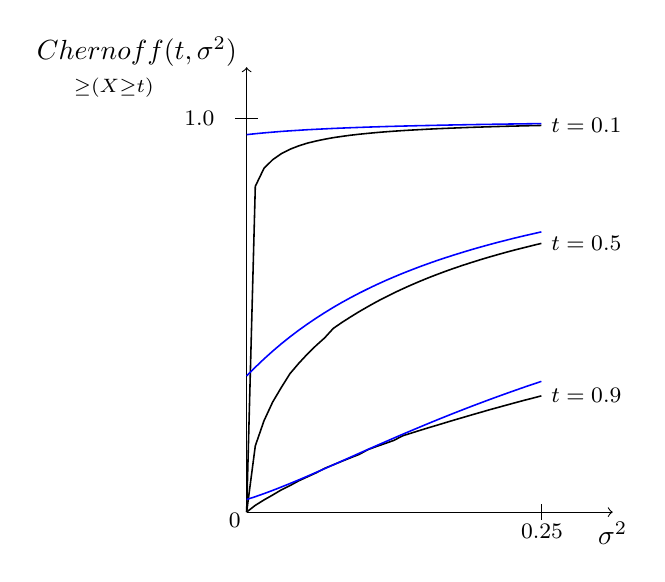
\begin{tikzpicture}[xscale=15, yscale=5]%[xscale=15, yscale=7.5]
\draw[->] (0,0) -- (0.31,0) node[anchor=north] {$\sigma^2$};
\draw[->] (0,0) -- (0,1.13) node[anchor=east, align=left] {$\text{Chernoff}(t,\sigma^2)$\\ $~~~~\scriptstyle\ge\pr(X\ge t)$};
\foreach \t in {0.1,0.5,0.9}{
	\draw[domain=0:0.25, color=black, line width=0.20mm, samples=35] 
		plot (\x,{((\x/(\x+\t))^(\x+\t)*(1.0/(1-\t))^(1-\t))^(1.0/(\x+1))}) node [right] {\footnotesize $t=\t$};
	\draw[domain=0:0.25, color=blue, line width=0.20mm, samples=35] 
		plot (\x,{e^(-\t*\t/(4*(1.0/17+\x/2)))}) node [right] {};
}

\draw (0.25,-0.02) -- (0.25,0.02);
\draw (-0.01,1) -- (0.01,1);
\draw	(0.25,-0.05) node{{\footnotesize $0.25$}}
		(-0.01,-0.02) node{{\footnotesize $0$}}
		(-0.04,1) node{{\footnotesize $1.0$}};
\end{tikzpicture}}
\end{figure}